\documentclass{article}
\usepackage{amsmath}
\usepackage{graphicx}

\title{Homework 13}
\author{Lucy Gschwantner}
\date{05.03.2023}

\begin{document}

\maketitle 
\pagebreak
\tableofcontents
\pagebreak

\section{8.138}
\subsection{a)}
\paragraph{Specification:}

Two forces $\vec{F_1}$, and $\vec{F_2}$, act at the same point. Determine the direction and
magnitude of the resultant force $\vec{F_R}$, and the angles that $\vec{F_1}$, and $\vec{F_2}$, 
make with $\vec{F_R}$ (forces in N).

\begin{equation}
   \vec{F_1} = \begin{pmatrix}
       6 \\ 
       4
   \end{pmatrix}, \vec{F_2} = \begin{pmatrix}
       8 \\ 
       1
   \end{pmatrix}, 
\end{equation}

\paragraph{Exercise:}

\begin{align}
    \vec{F_R} &= \vec{F_1} + \vec{F_2} \\ 
    \vec{F_R} &= \begin{pmatrix}
    14 \\ 
    5
    \end{pmatrix} \\[10pt]
    \hline
    \noalign{\vskip 10pt}
    |\vec{F_R}| &= \sqrt{14^2 + 5^2} \\
    |\vec{F_R}| &= \sqrt{221} \\[10pt]
    \hline
    \noalign{\vskip 10pt}
    \cos(\alpha) &= \frac{\vec{F_1} \cdot \vec{F_R}}{|\vec{F_1}| * |\vec{F_R}|} \\
    \cos(\alpha) &= \frac{104}{107.200746266} \\
    \alpha &= \arccos(0.970142500146) \\
    \alpha &= 14.03624^\circ \\[10pt]
    \hline
    \noalign{\vskip 10pt}
    \cos(\beta) &= \frac{\vec{F_2} \cdot \vec{F_R}}{|\vec{F_2}| * |\vec{F_R}|} \\
    \cos(\beta) &= \frac{117}{119.854077945} \\
    \beta &= \arccos(0.976187060182) \\
    \beta &= 12.52881^\circ
\end{align}

\paragraph{Answer:}
The direction of $\vec{F_R}$ is $\begin{pmatrix}
   14 \\ 
   5
\end{pmatrix}$ and its magnitude is $\sqrt{221}N$, the angle $\alpha$ between $\vec{F_1}$ 
and $\vec{F_R}$ is $14.03624^\circ$ and the angle $\beta$ between $\vec{F_2}$ and $\vec{F_R}$ 
is $12.52881^\circ$.

\pagebreak

\section{8.43}
\paragraph{Specification:}
A sled is pulled along a distance $s$ by a rope with a constant force $\vec{F}$. The sled
is pulled by the rope. The rope forms an angle $\phi$ with the horizontal surface.

\subsection{b)}
\paragraph{Requirements:}
Calculate the direction of the force and the amount of work $W$ done while pulling.

\begin{equation}
   s = 2.3km; F = |\vec{F}|  = 55N; \phi = 32^\circ 
\end{equation}

\paragraph{Exercise:}
\begin{align}
    \vec{F_x} &= 55\cos(\phi) \\
    \vec{F_x} &= 46.6426441414 \\
    \vec{F_y} &= 55\sin(\phi) \\
    \vec{F_y} &= 29.1455613688 \\[10pt]
    \vec{F} &= \begin{pmatrix}
        46.6426441414 \\
        29.1455613688 \\ 
    \end{pmatrix} \\[10pt]
    \hline 
    \noalign{\vskip 10pt}
    W &= \vec{F_x} * s \\
    W &= 46.6426441414N * 2300m \\
    W &= 107278.081525 Nm
\end{align}

\paragraph{Answer:}
The force $\vec{F}$ is $\begin{pmatrix}
        46.6426441414 \\
        29.1455613688 \\ 
    \end{pmatrix}$ and the Work done while pulling the sled on the ground is $107278.081525 Nm$. 

\pagebreak

\section{8.44}
\subsection{a)}

\paragraph{Specification:}
A body is pulled in the direction of $\vec{r}$ on a distance $s$ with the gradient $k$ by a
force $\vec{F}$.

\paragraph{Requirements:}
Calculate the work done in the process ($F = |\vec{F}|$).

\begin{equation}
   s = 650m; k = 10\%; F = 65N; \vec{r} = \begin{pmatrix}
       5 \\ 
       12
   \end{pmatrix} 
\end{equation}

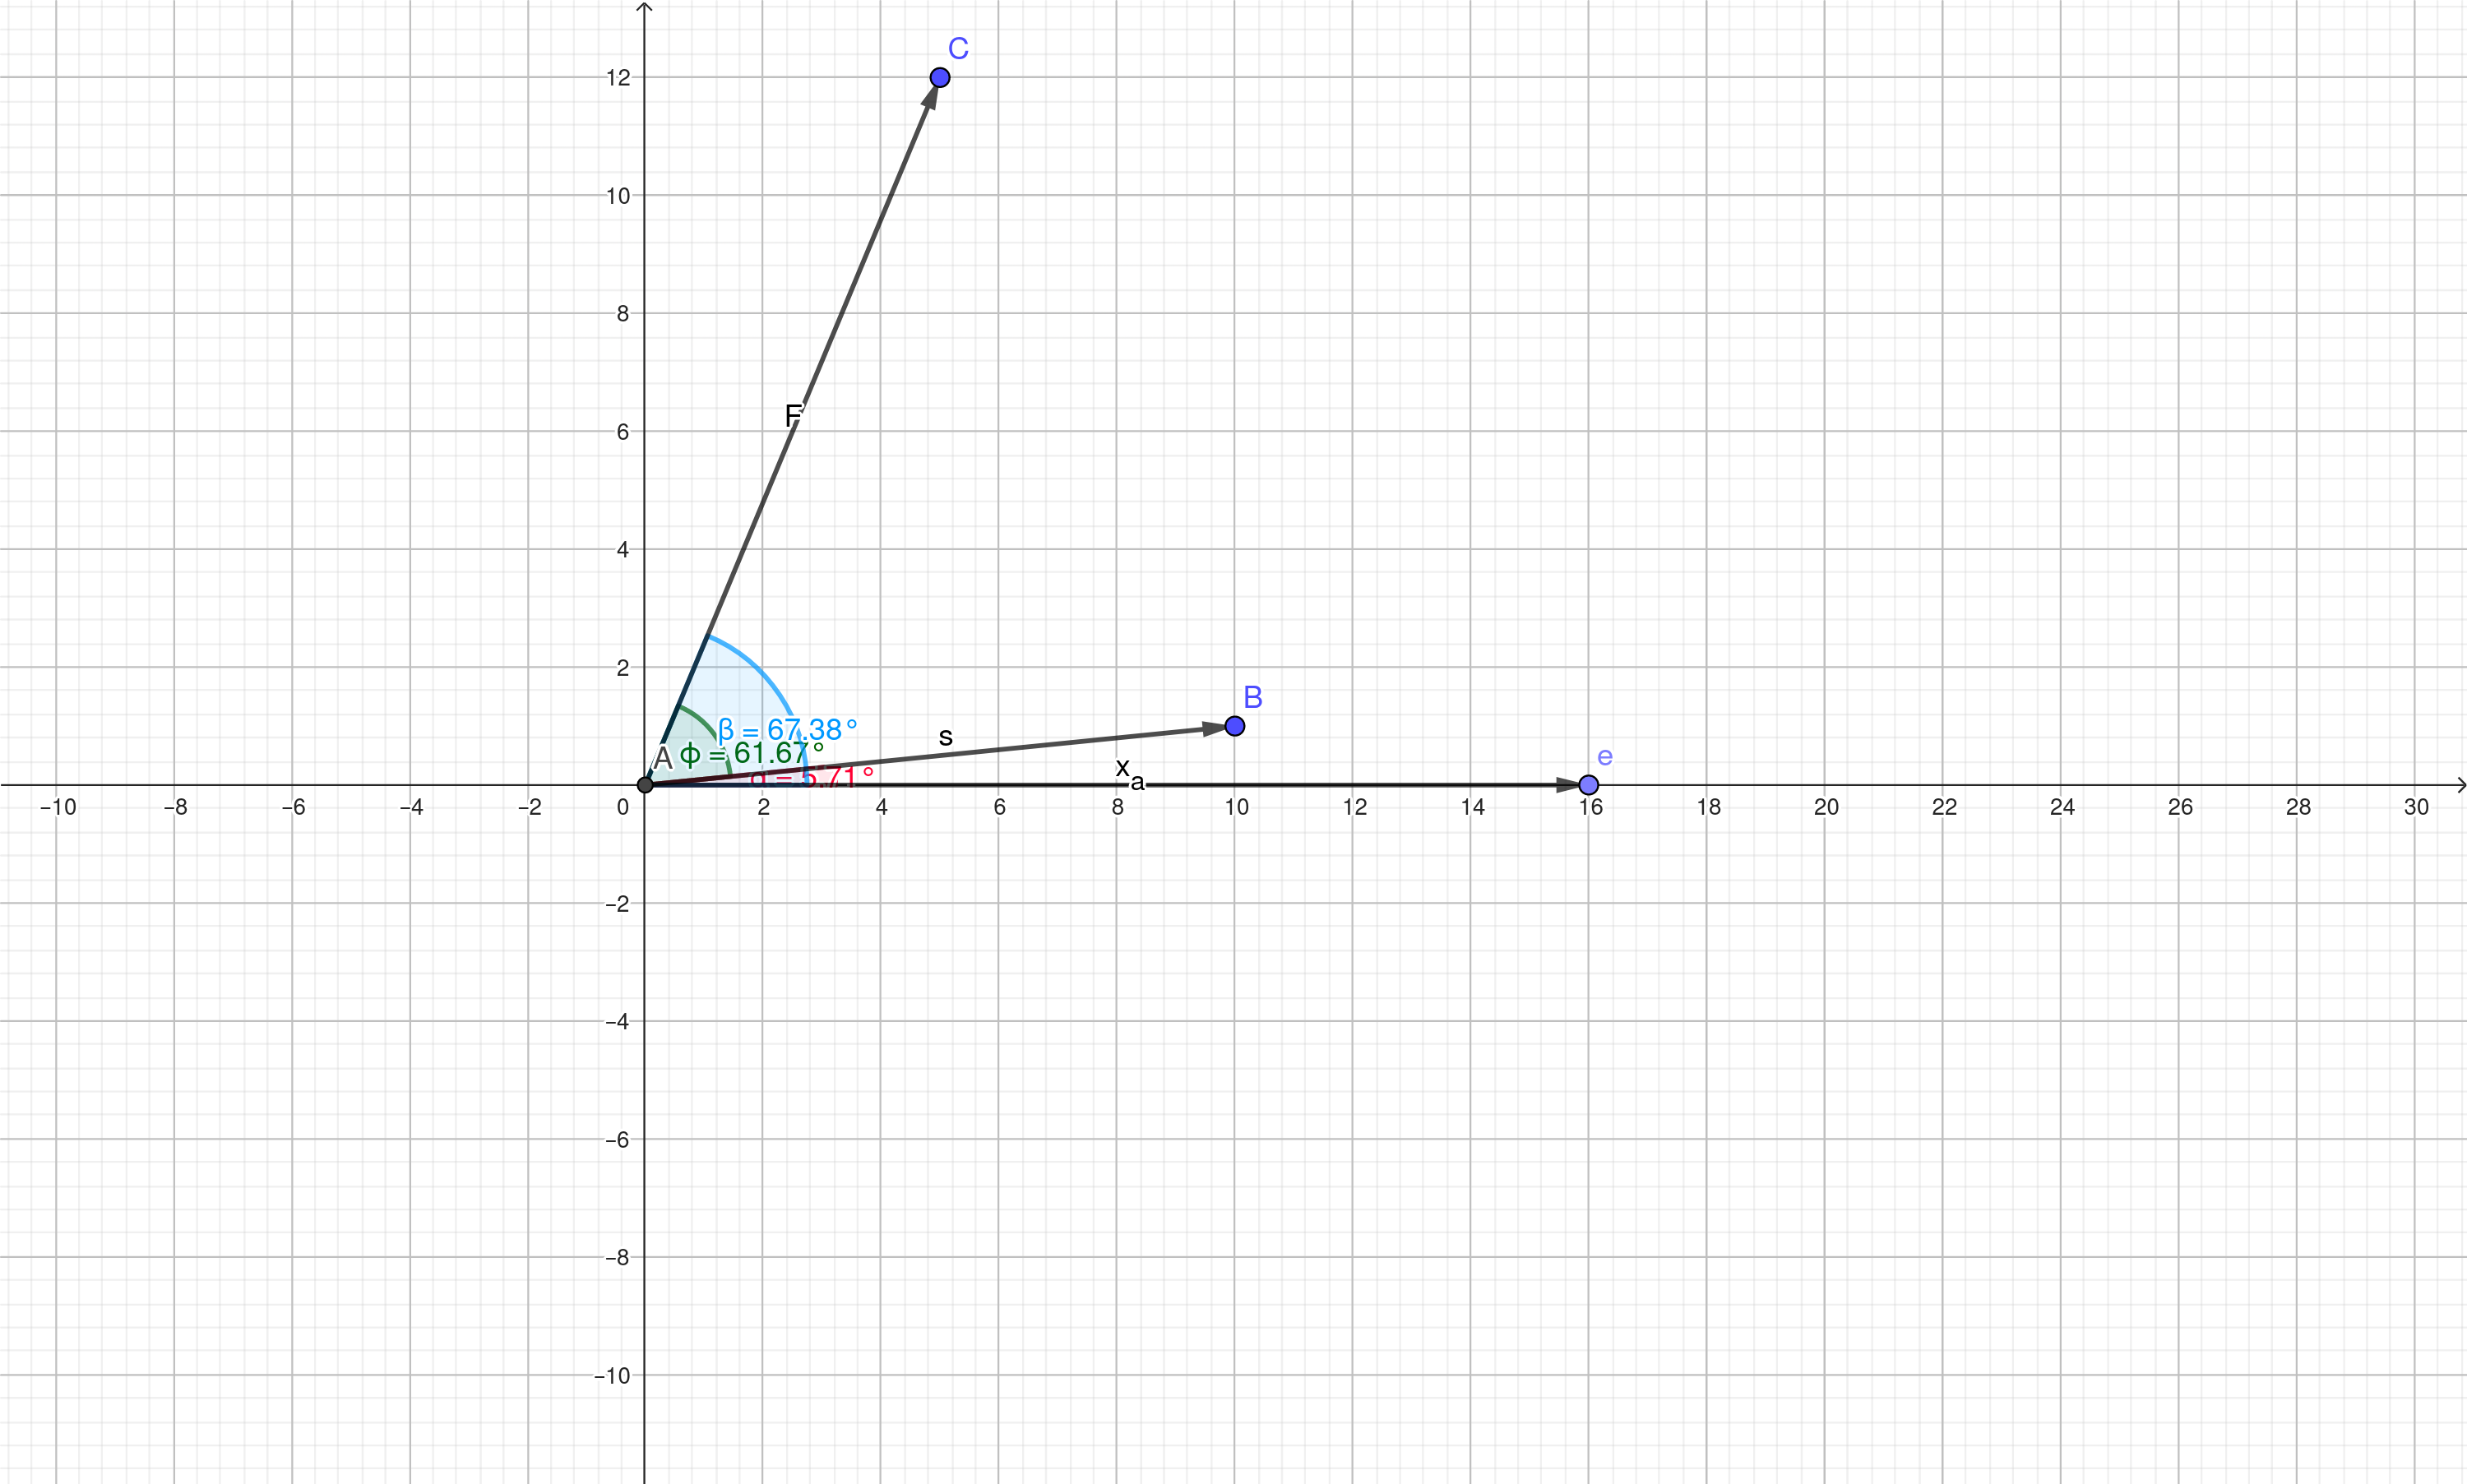
\includegraphics[width=\linewidth]{images/8-44-a.png}

\paragraph{Exercise:}

\begin{align} 
    \phi &= \beta - \alpha \\
    W &= \cos(\phi)*F*s \\[10pt]
    \hline 
    \noalign{\vskip 10pt}
    \cos(\beta) &= \frac{\vec{r_x}}{|\vec{r}|} \\
    \beta &= \arccos(\frac{5}{13}) \\
    \beta &= 67.38014^\circ \\[10pt]
    \alpha &= \arctan(\frac{1}{10}) \\
    \alpha &= 5.7105931375^\circ \\[10pt]
    \hline 
    \noalign{\vskip 10pt}
    \phi &= 67.38014^\circ - 5.7105931375^\circ \\
    \phi &= 61.6695468625^\circ \\[10pt]
    W &= \cos(61.6695468625^\circ) * 65 * 650 \\
    W &= 20049.9828187
\end{align}

\paragraph{Answer:}
$20049.9828187Nm$ are done in the process of pulling the body.

\end{document}
